% load TENOR file template

% hfmt-drawsocket
% -----------------------------------------------
% Template for SMAC SMC 2013
% adapted and corrected from the template for SMC 2012, which was adapted from that of SMC 2011
% further updated for TENOR 2015, 2016, 2017 and 2018
% -----------------------------------------------
\documentclass{article}
\usepackage{tenor2019}
\usepackage{ifpdf}
\usepackage[english]{babel}
\usepackage{balance}
\usepackage{listings}
\usepackage{float}

%%%%%%%%%%%%%%%%%%%%%%%% Some useful packages %%%%%%%%%%%%%%%%%%%%%%%%%%%%%%%
%%%%%%%%%%%%%%%%%%%%%%%% See related documentation %%%%%%%%%%%%%%%%%%%%%%%%%%
%\usepackage{amsmath} % popular packages from Am. Math. Soc. Please use the 
%\usepackage{amssymb} % related math environments (split, subequation, cases,
%\usepackage{amsfonts}% multline, etc.)
%\usepackage{bm}      % Bold Math package, defines the command \bf{}
%\usepackage{paralist}% extended list environments
%%subfig.sty is the modern replacement for subfigure.sty. However, subfig.sty 
%%requires and automatically loads caption.sty which overrides class handling 
%%of captions. To prevent this problem, preload caption.sty with caption=false 
%\usepackage[caption=false]{caption}
%\usepackage[font=footnotesize]{subfig}



% paper title, authors
\def\papertitle{Massive Networked Music Performance in the Old Elbe Tunnel
}
\def\firstauthor{first author} % Georg Hajdu
\def\secondauthor{second author} % Rama Gottfried

\def\Hochschule{ Hochschule f\"ur Musik und Theater}

\title{\papertitle}
\twoauthors
   {\firstauthor} {	
      Hochschule f\"ur Musik und Theater\\
         Hamburg, Germany \\ %
   \small{\tt \href{mailto:georg.hajdu@hfmt-hamburg.de}{georg.hajdu@hfmt-hamburg.de}}}
    {\secondauthor} {
   Hochschule f\"ur Musik und Theater\\
   Hamburg, Germany \\ %
   \small{\tt \href{mailto:rama.gottfried@hfmt-hamburg.de}{rama.gottfried@hfmt-hamburg.de}}}


% other setup

%user defined variables


%\hyphenpenalty10000

\usepackage{xspace}
\def\symbolist{\textsc{symbolist}\xspace}
\def\drawsocket{\textsc{drawsocket}\xspace}
\def\maxscore{\textsc{maxscore}\xspace}
\def\innovativ{Innovative Hochschule: \textit{Stage\textunderscore2.0}\xspace}

\def\oscfontsize{\footnotesize}

\def\oscformat{
  mathescape,
  columns=fullflexible,
  basicstyle=\oscfontsize\fontfamily{lmvtt}\selectfont 
}

\makeatletter
\newcommand{\verbatimfont}[1]{\renewcommand{\verbatim@font}{\ttfamily#1}}
\makeatother


% adds the automatic
% Saves a lot of ouptut space in PDF... after conversion with the distiller
% Delete if you cannot get PS fonts working on your system.

% pdf-tex settings: detect automatically if run by latex or pdflatex
\newif\ifpdf
\ifx\pdfoutput\relax
\else
   \ifcase\pdfoutput
      \pdffalse
   \else
      \pdftrue
\fi

\ifpdf % compiling with pdflatex
  \usepackage[pdftex,
    pdftitle={\papertitle},
    pdfauthor={\firstauthor, \secondauthor},
    bookmarksnumbered, % use section numbers with bookmarks
    pdfstartview=XYZ % start with zoom=100% instead of full screen; 
                     % especially useful if working with a big screen :-)
   ]{hyperref}
  %\pdfcompresslevel=9

  \usepackage[pdftex]{graphicx}
  % declare the path(s) where your graphic files are and their extensions so 
  %you won't have to specify these with every instance of \includegraphics
  \graphicspath{{./figures/}}
  \DeclareGraphicsExtensions{.pdf,.jpeg,.png}

  \usepackage[figure,table]{hypcap}

\else % compiling with latex
  \usepackage[dvips,
    bookmarksnumbered, % use section numbers with bookmarks
    pdfstartview=XYZ % start with zoom=100% instead of full screen
  ]{hyperref}  % hyperrefs are active in the pdf file after conversion

  \usepackage[dvips]{epsfig,graphicx}
  % declare the path(s) where your graphic files are and their extensions so 
  %you won't have to specify these with every instance of \includegraphics
  \graphicspath{{./figures/}}
  \DeclareGraphicsExtensions{.eps}

  \usepackage[figure,table]{hypcap}
\fi

%setup the hyperref package - make the links black without a surrounding frame
\hypersetup{
    colorlinks,%
    citecolor=black,%
    filecolor=black,%
    linkcolor=black,%
    urlcolor=black
}



\begin{document}
%

\capstartfalse
\maketitle
\capstarttrue
%
\begin{abstract}
In this paper we present a new distributed score display system currently under development at the Hochschule f\"ur Musik und Theater, Hamburg.
The project was initiated as part of a large-scale live performance in the St. Pauli Elbe tunnel (sometimes also referred to as Old Elbe Tunnel), for 144 musicians spread out over the 864 meters of its two tubes.
We describe here the background of this project and the current status of the technological and musical considerations required to achieve this event.

\end{abstract}

\section{Introduction}\label{sec:intro}

%why did we need to make this system?
%introduce the St. Pauli project
%ensemble performance 
%
%
%Definition of Situative Performance
%
%Quintet.net and the European Bridges Ensemble

In a presentation on his piece Music for a Wilderness Lake (1979), R. Murray Schafer referred to it as a ``music for a place (personal communication).'' 
This music greatly depends on the topology of the environment it is performed in. While cases of topologically informed music (with static and/or moving musicians) have already existed in since the 1500’s with renewed interest in the 19th century (in his Memos Charles Ives tells the story of his father experimenting with marching bands walking towards each other and playing different tunes), it became more of a practice during the second part of the 20th century. Examples include Musik f\"ur ein Haus (Stockhausen, 1968), Eine Brise / Fl\"uchtige Aktion f\"ur 111 Fahrr\"ader (Kagel, 1996), music by Alvin Curran who created music performed in the Sydney harbor or on the river Thames, among other places.

One of the difficulties of such a practice is maintaining synchronicity, as the participants either act on their own or execute scores with little coordination amongst each other due to lack of visual and auditory cues from a central agent / conductor. Such difficulties are aggravated if the location of the performance is a virtual one such as in networked music performance (NMP). Recent developments in digital technologies have leveraged some if not all of these difficulties by providing audiovisual tools. They are either capable of creating a shared space by low-latency streaming or the exchange of control messages. While audio/video streaming has yielded excellent results since the early 2000s  (e.g. JackTrip~\cite{caceres2010jacktrip}), systems that feature music notation in networked environments have been rare and only become more widespread since about 2010. Quintet.net~\cite{hajdu2005quintet}, a networked multimedia performance environment developed by Georg Hajdu is an earlier example of software in which the interaction of musicians is facilitated by a visual notation layer. The European Bridges Ensemble was an ensemble for NMP whose members have been  focussing on creating scores capable of capturing the specificities of a particular performance scenario. ``Situative scoring'' is a term coined by Sandeep Bhagwati~\cite{bhagwati2017vexations} describing scores that are defined as scores that deliver time- and context-sensitive score information to musicians at the moment when it becomes relevant.... Lately, reactive, interactive, locative scores have added new options to situative scoring.''

In this paper we are describing the musical and technological prerequisites for a project dubbed Symphony for a Tunnel to be realized in Hamburg in May of 2019. The Old Elbe Tunnel is a remarkable landmark in the heart of the Hamburg port. Completed in 1911, it was considered a technological marvel at the time, connecting two neighborhoods below the Elbe river. Featuring two tubes for pedestrians, cyclists and automobiles which are being carried down / up by sizeable lifts to / from the bottom 24m beneath the surface, it is also an extraordinary place for performances. Its Jugendstil half cylinders form a resonant body in which the sound of a single instrument carries over large distances with relatively little decay \footnote{In an experiment featuring a violin playing scales at mezzo forte dynamics, it could be heard at 50m distance as if it was still be played right next to the observer}.

The Stage\_2.0 grant within the Innovative Hochschule initiative of the Federal Ministry of Education and Research in Germany (BMBF) has finally laid the financial foundation for a musical project in the tunnel. The aim is to connect a large number of musicians via a network of connected devices delivering scores on time. We went through a number of scenarios until zooming in on the most practical solution: As the total circular length of the tunnel is about 860 m and an ideal spacing of individual musicians was determined by us to be around 5 to 6 m, it was a most welcome finding that dividing 864 by 6 yielded 144, a highly divisible number with technical and compositional repercussions. For instance, this number allowed us to define identical sub-groups consisting of 12 musicians each or to place 8 access points at regular distances between musicians (see Figure \ref{fig:Elbtunnel_GrundrissVers2}). An older, safer idea consisting of tablet computers connected to a wired Ethernet network was abandoned in favor of a Wi-Fi network as it would have required anywhere between 2.5 and 5 km of cables depending on the number of switches involved. 
Another serendipitous finding was that when Rama Gottfried joined the Stage\_2.0 project in 2018, he had already been working on a node.js-based system for the Berlin Ensemble Mosaik and possessed the expertise to take on a project that would also take advantage of Cycling ’74’s recent effort to integrate node.js into their Max multimedia authoring environment.


% \innovativ


\section{Foundations} \label{sec:foundations} 
%
%Conected prior work
%  
%Maxscore \cite{didkovsky2008maxscore}
%
%Max Mira system
%
%Symbolist (related to SVG/OSC work) \cite{gottfried2018symbolist, gottfried2015svg}


%node.js prototypes used for ensemble mosaik

A small number of software solutions are capable delivering scores in a networked environment, most notably InScore~\cite{fober2013programming}, bach~\cite{agostini2015max} and MaxScore~\cite{didkovsky2008maxscore}. MaxScore emerged from the ongoing effort to provide a robust notation layer to the Quintet.net multimedia performance environment and has first been used in 2007 in a performance at the Budapest Kunsthalle. MaxScore went through several iterations and incarnations (e.g. as LiveScore bringing standard music notation to the Ableton Live DAW).
For clarity’s sake we will now use the following nomenclature: MaxScore denotes the environment consisting of numerous objects, abstractions and scripts while the name MaxScore object refers to the Max Java object called \linebreak com.algomusic.max.MaxScore. The MaxScore object is based on JSML, a language developed by Nick Didkovsky. In contrast to other Max notation solutions it requires a canvas to which to draw to and receive mousing information from. This “division of labor” affords greater flexibility as it allows the MaxScore object to render to various targets, such as Max drawing objects (lcd, jsui, jit.mgraphics) as well as SVG and PNG files, the latter via Jitter matrix export). Drawing commands, specific to the environment they are being executed in, can be defined as rendered messages and attached to notes, staves or measures. 

In a 2018 TENOR paper, Hajdu and Didkovsky described how scores generated by MaxScore could be displayed in real-time on iPads and browsers via the Max Mira and MiraWeb systems (footnote: reference to Carey and Hajdu: NetCanvas). This approach relies on the Max fpic object which can be mirrored on handheld devices. Having to create a PNG of the entire score each time it changes and using Mira’s and MiraWeb’s TCP and/or web socket connections for upload seemed like crutch and mandated a more elegant approach harnessing the power of modern browser with their JavaScript/HTML 5/SVG implementations. Our efforts thus led to the development of hfmt.drawsocket, which is a robust node.js-based solution allowing on-time delivery of scores that can be scaled and animated without loss of quality (due to the use of vector graphics). 






\section{Drawsocket}
The \drawsocket system consists of a Node.js server running inside a Max abstraction called hfmt.drawsocket.
Using the NodeForMax environment, the server functions to relays messages from a Max patch to client browsers, routed to individually addressable channels based on the browsers' URL. {\color{red} See our other paper}.
The server uses the URL as an OpenSoundControl (OSC) address prefix, which tags messages with a target destination.
When new drawing commands are received by the server, the commands are routed to the client browsers via WebSockets.
On receiving new messages from the server, the client parses the data and uses it to produce new display information in the browser, using Scalable Vector Graphics (SVG) as the main display format.
The system also provides tools for animation of graphic elements, as well as user interaction callbacks, among other features.
With this system in place, MaxScore connects through the hfmt.drawsocket Max abstraction to the client browsers, and then renders its score for each remote location based on the OSC address prefix.







\begin{figure*}[h]
    \centering
    \begin{minipage}{0.45\textwidth}
        \centering
        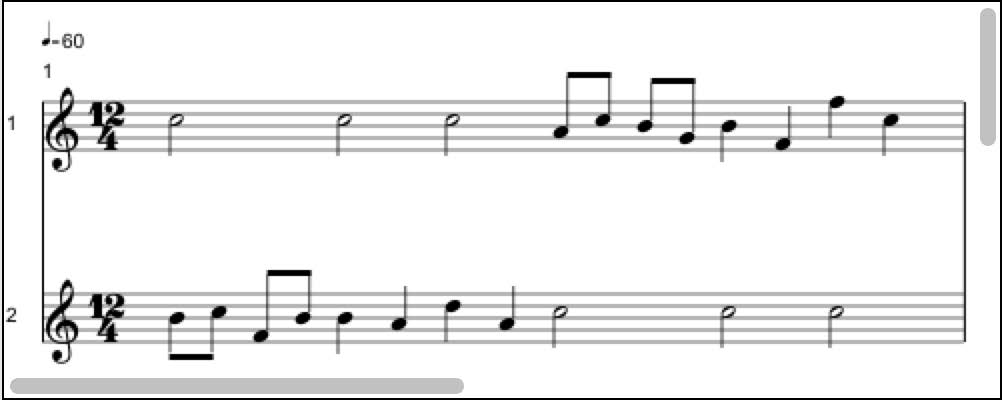
\includegraphics[width=0.9\textwidth]{Tenor-Paper-6.jpg} 
                \caption{A score with a random melody rendered in MaxScore’s default layout.
        \label{fig:Tenor-Paper-6}}
    \end{minipage}\hfill
    \begin{minipage}{0.45\textwidth}
        \centering
        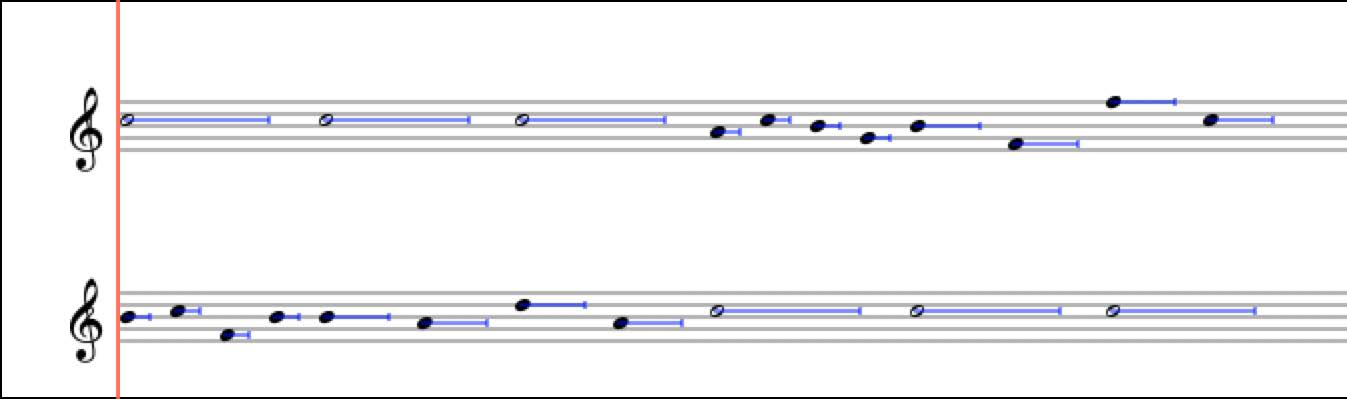
\includegraphics[width=1\textwidth]{Tenor-Paper-7.jpg} 
       	\caption{Same score after applying proportional notation. The default hold times indicated by the blue line is set to 80\% of the event’s nominal duration.
\label{fig:Tenor-Paper-7}}
    \end{minipage}
\end{figure*}

\section{Maxscore}
As mentioned in section~\ref{sec:foundations}., MaxScore possesses a fair amount of flexibility in terms of rendering to a wide array of targets. The JavaScript object render2Browser.js was created to facilitate the communication between the MaxScore object and the hfmt.drawsocket abstraction. The js object was designed with MNMP in mind. Such performances pose enormous difficulties when distributing large scores with dozens of staves. In performances with Quintet.net, scores containing just a few staves were split into instructions to be reassembled by individual instances of the MaxScore object and rendered locally by the Clients. But doing the same with dozen of instances (potentially destabilizing the environment and introducing unwanted latency), we resorted to a different strategy by implementing the concept of multi-client rendering, treating the ensemble of clients like one single canvas. In Maxscore, nearly every rendering message contains indexes referring to the notation object it represents  (Figure~\ref{fig:maxscore-mesages}). Thanks to those indexes, render2Browser.js is capable of dynamically reroute a rendering message to targets set by the staffgroups attribute. This attribute can have the following values: score, parts or a list containing either indexes (for individual staves), two indexes joined by hyphens (for a staff range) or any number of indexes joined by plusses (for arbitrary collections of staves) such as in this example: staffgroups 0 1-2 2 0+3.

In addition to splitting and routing messages, the object is also capable of respacing staves so that resulting layout looks acceptable. It does so by querying the MaxScore object during rendering to obtain crucial information about staff spacing and using this information to apply offsets to the y values of each message to be rendered.




\begin{figure}[h]
\centering
\begin{lstlisting}[ mathescape,
						columns=fullflexible,
						basicstyle=\oscfontsize\fontfamily{lmvtt}\selectfont,
						breaklines=true,
						 frame=single ]
tempoqtrequals 20. 21. 0.5 Measure 0. ...
tr 22. 75.959999 0.5 Staff 0. 0. staffnumber1 0. 63. 0.5 Staff 0. 0. timesig4 43. 57. 0.5 Staff 0. 0.
...
StaffLine 0. 0. 4. 0.5 20. 75. 300.660797 75. false
...
frgb 0 0 0
noteheadblack 83.620689 57. 0.5 Note 0. 0. 0. 0.
frgb 0 0 0
no_accidental 75.555557 57. 0.5 Note 0. 0. 0. 0.
frgb 0 0 0
stem 76.620689 79. 0.5 Note 0. 0. 0. 0. STEM_DOWN
RenderMessage staff 0 0 166. 13. 0.5 
rendered Picster-Element[5] 175.3ocUOsnBBCCCzOk6dAg[...]
\end{lstlisting}

\caption{A sample of rendering messages generated by the MaxScore object. 
\label{fig:maxscore-mesages}}
\end{figure}

Figure \ref{fig:maxscore-mesages} shows a sample of rendering messages generated by the MaxScore object. Note that nearly every message is accompanied by indexes (in red) referring to the notation object they represent. The y coordinates (blue numbers) are remapped according to the current staffgroups setting. The RenderMessage message contains a gzip’ed JSON object which in turn codes for a graphical score element such as a line, a rectangle, an arc or an image.

render2Browser.js is also capable of animating any number of cursors moving across set of measures and staves (see TENOR 2018 paper).

\begin{figure}[h!]
        \centering
        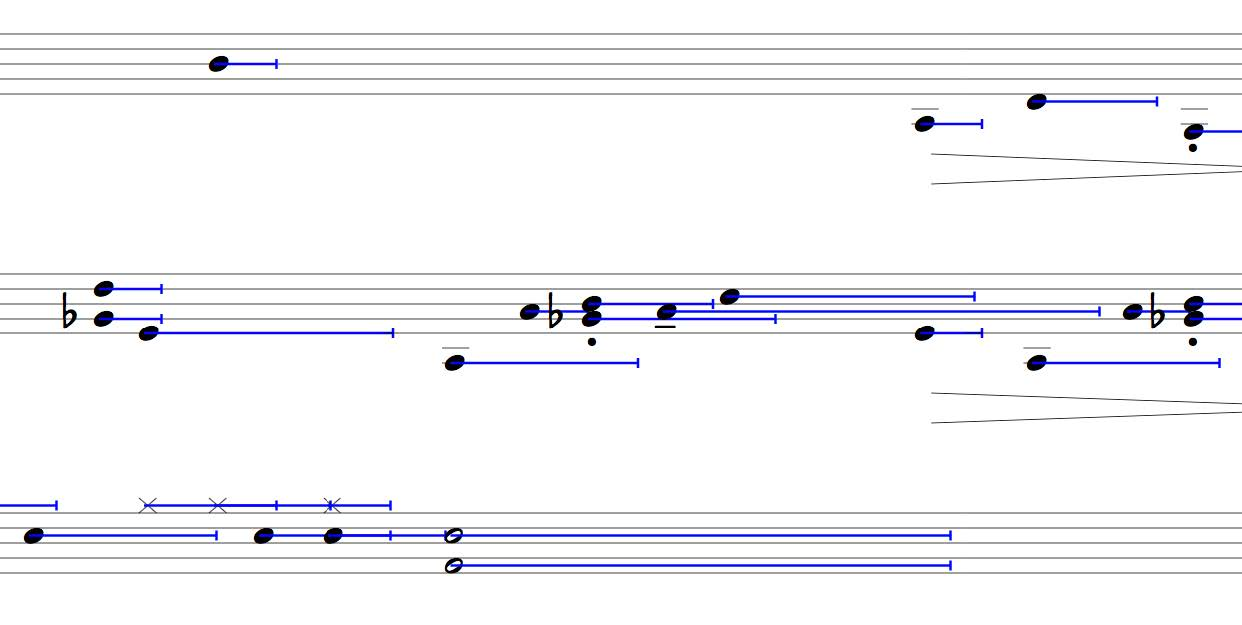
\includegraphics[width=0.4\textwidth]{Tenor-Paper-8.jpg} 
       	\caption{Excerpt from Raindrops Keep Falling (2018) for clarinet, cello, drum set and multimedia.
\label{fig:Tenor-Paper-8}}
\end{figure}


\begin{figure*}[h]
        \centering
        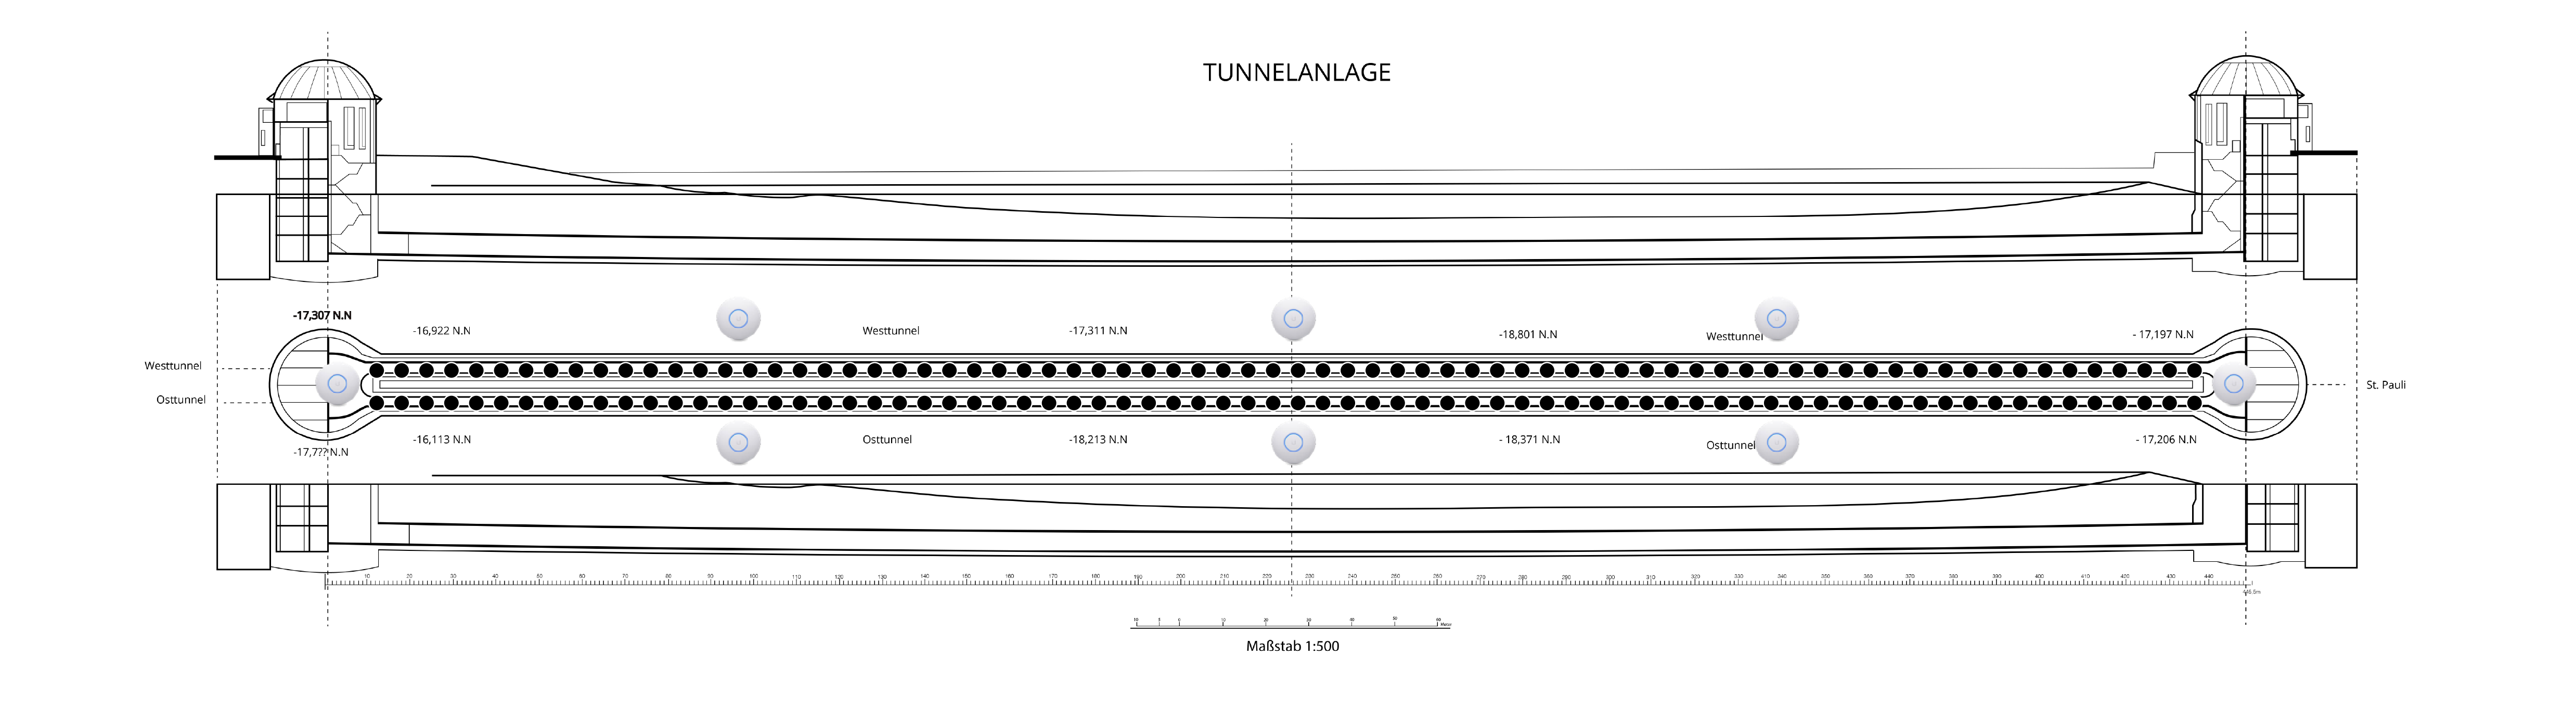
\includegraphics[width=1\textwidth]{Elbtunnel_GrundrissVers2.png} 
       	\caption{Cross section and top view of the Old Elbe Tunnel. Eight access points will be spaced at regular distances, each providing coverage for 18 players.
\label{fig:Elbtunnel_GrundrissVers2}}
\end{figure*}

\begin{figure*}[h]
        \centering
        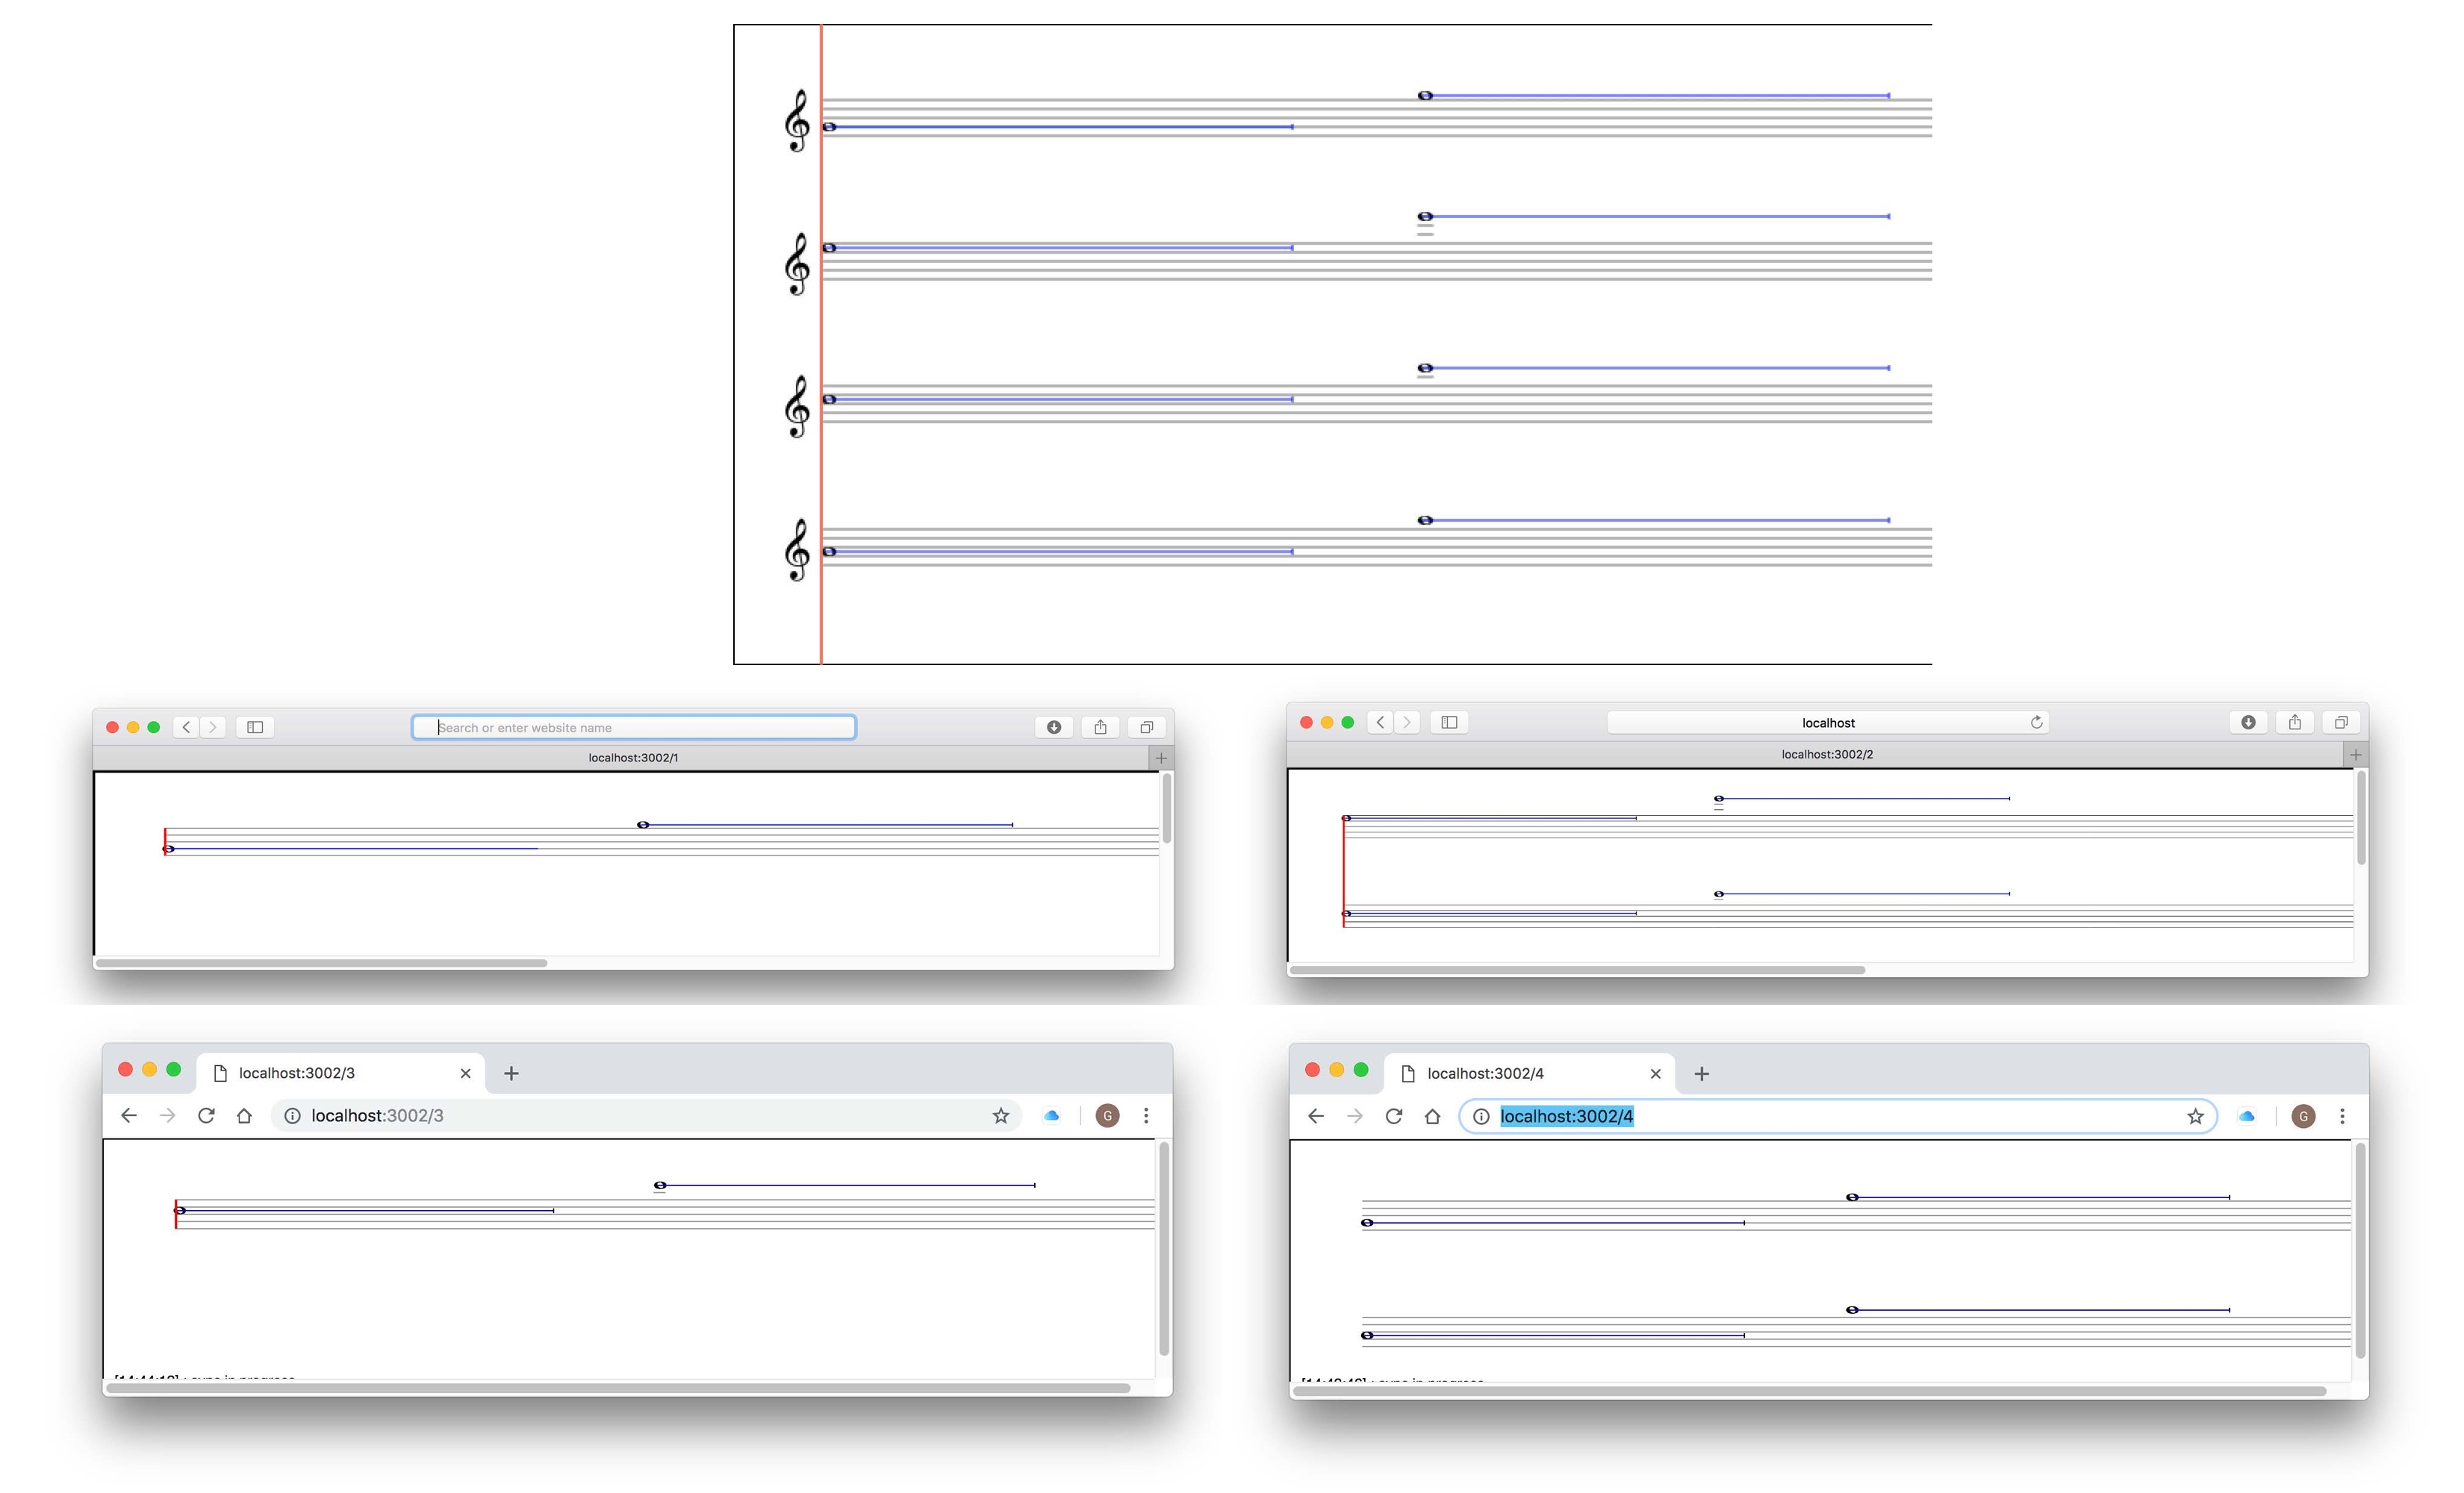
\includegraphics[width=1\textwidth]{Tenor-Paper.png} 
       	\caption{A MaxScore score with 4 staves (top) rendered dynamically in four browser windows (center and bottom). The staves are split and grouped by render2Browser.js according to the following staffgroup settings: 0 1-2 2 0+3.
\label{fig:Tenor-Paper}}
\end{figure*}

To scroll the entire score horizontally, we created another JavaScript object called maxscore.proportionalNotation.js. It toggles between MaxScore’s default score layout and its proportional representation by hiding rests, stems, beams and naturals and indicating the duration of a note by a line extending from a note. The length of a measure is calculated by obtaining its tempo and time signature values and taking a setTimeUnit attribute into consideration. The durational scaling base value of 0.385 has proven to be optimal for spatially representing the delta time between events. The start message will cause a playhead to appear at the position given by the scoreLeftMargin attribute and instruct the browser to scroll the score. We are planning to also support scores created for the Decibel ScorePlayer in the future. 



%describe use of hfmt.drawsocket via Maxscore translation script.
\section{Setup in the Elbe tunnel}
The planned performance system for the Elbtunnel performance consists of a central server running the MaxScore/ Drawsocket framework, and eight Ubiquiti Unifi WIFI access points providing robust and redundant coverage within the tunnel. The APs will be connected to the network by switches linked via fiberoptic cables to overcome the limitations of current Ethernet cables.
Each of the 144 performers will have a iPad mounted on a music stand, connected to a unique URL-OSC routing prefix (e.g. {/1}, {/2}, {/3}, ..., {/144} ). 

There will be 4 concerts on two days with pieces written by established composers as well as HfMT multimedia students. The tunnel will be blocked off for the general public and the audience will be allowed to freely move around during the performance.





\section{Case study}

A performance  at the December 2018 WOCMAT conference in Hsinchu, Taiwan posed an excellent opportunity to test drive the software at its current state.
A new piece (Raindrops Keep Falling) by Georg Hajdu for clarinet, cello and percussion with multimedia consists of a transition between various rain samples and a late-1960’s hit called Raindrops Keep Fallin' On My Head mediated by a Max Pluggo effect called Raindrops. \footnote{It’s also a tongue-in-cheek reference to the usual end-of-year weather pattern in Taiwan.} The piece features 12 different versions of the song found on the Internet. The HfMT graduate student and research assistant James Cheung arranged the songs in such manner that they all share the same tempo structure and key signature, allowing the seamless navigation between those versions. James also created an arrangement of the song for the aforementioned instrumentation to be performed simultaneously with the recording, which was further subject to processing. First, parts of the score were “whited out” by a probabilistic process so that more and more events were allowed to appear paralleling a similar process applied to the audio tracks. The whiting-out was achieved by a JavaScript object called maxscore.whiteout.js capable of applying a “whiteout” gradient to a given section (the name was inspired by Cat Hope’s piece The Great White). Second, the score was turned into proportional notation, transmitted to the iPads of the performers via hfmt.drawsocket and scrolled in synch with the audio. The system held up to its promise as a computer-based conducting system. The scrolling was fluid and the musicians stayed in tempo despite the tempo fluctuations in the audio track. 





\section{Future Work}
We expect the Old Elbe Tunnel to be a test bed for situative performances of orchestral dimensions. This project will be further developed according to the following criteria: 
1. The situative aspect: The system can be scaled to other outdoors and indoors settings with unique topologies. Once the system has proven its robustness, we will  most likely see more real-time and interactive uses.
2. The assistive aspect: Allowing semi-professional and amateur musicians to participate in large-scale events with little prior orchestra experience. A transcription of Ligeti's Atmospheres into proportional notation, for instance, could leverage some of the difficulties reading the complex notation in rehearsals and concerts. The networked notation tool SmartVox by Jonathan Bell and Benjamin Matuszewski \cite{bell2017smartvox} has already yielded excellent results working with amateur and student choirs. Cat Hope's opera Speechless is another case where a networked notation tool (Decibel Score Player) has been used in large scale performance.

\begin{acknowledgments}
The authors would like to thank James Cheung for their detailed testing the system which pushed the development of many new features and design considerations. We would also like to acknowledge the Federal Ministry of Education and Research in Germany (BMBF), for their support of this research through the Innovative Hochschule: Stage\_2.0 initiative.
\end{acknowledgments} 

%%%%%%%%%%%%%%%%%%%%%%%%%%%%%%%%%%%%%%%%%%%%%%%%%%%%%%%%%%%%%%%%%%%%%%%%%%%%%
%bibliography here
\balance
\bibliography{symbolist}
\end{document}




